\chapter{Clouds}\label{chp:LABEL_CHP_4}

One of the main applications of Ray Marching is in the rendering of realistic smoke, clouds, which are called volumetric objects. Clouds are mostly made of two main high-albedo types of particles, if not considering dirt or other minimal particles: air and water/ice. \cite{:REF_IN_1}
Since clouds are not solid, when light hits them, some rays bounce, but some go through the object. Not only that, the water particles are anisotropic\cite{:REF_IN_1}, which means that light tends to bounce differently depending on the direction from which it hits the cloud. All in all, there is a lot to adapt from the original Ray Marching concocted. 

\section{Volumetric Rendering}

Firstly, to render gaseous materials, instead of avoiding going into surfaces, Ray Marching needs to go through the clouds. For that, the SDF now represents density instead of "distance to surface". For the sake of clarity, the SDFs are inversed so that the distance to a point is as follows. 

\begin{itemize}
    \item Outside of the primitive, yields a negative density, or no density.
    \item Inside of the primitive, yields a positive density, and the further the point is from bounds, the higher the density is.
\end{itemize}

Secondly, to consistently sample the density along the cloud, a constant step size is better suited - instead of querying the scene's distance for the next marching step, each step will perform a constant size.

\begin{algorithm}[H]
\caption{MarchRay}
\label{alg:marchray}
\begin{algorithmic}[1]
\Procedure{MarchRay}{RayOrigin, RayDirection, Scene}
    \State $ \mathbf{MarchDistance} \gets \text{0} $
    \State $ \mathbf{Hit} \gets \text{NULL\_HIT} $
    \State $ \mathbf{IsHit} \gets \text{false} $
    \For {$step \gets 0$ to $\text{MAX\_MARCH\_STEPS} - 1$}
        \State $\mathbf{MarchPos} \gets  RayOrigin+ (MarchDistance * RayDirection) $
        \State $\mathbf{Hit} \gets \Call{GetDistance}{MarchPos, scene}$
        \If{$\text{Hit.distance} < \text{SURFACE\_DISTANCE}$}
            \State $ \mathbf{IsHit} \gets \text{true} $
            \State $ break $
        \EndIf
        \If{$\text{MarchDistance} > \text{MAX\_MARCH\_DISTANCE}$}
            \State $ break $
        \EndIf
    \EndFor
    \State \Return $\mathbf{Hit}$
\EndProcedure
\end{algorithmic}
\end{algorithm}


\section{Noise}



\section{Volumetric Shading}

% \begin{figure}[ht]
%     \centering
%     \fbox{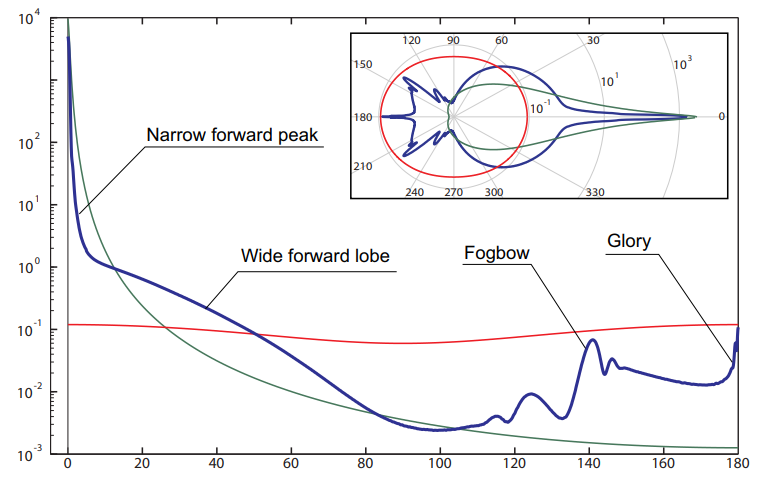
\includegraphics[width=9.5cm]{imagens/phase_functions.png}}
%     \caption{Log plots (inset: polar log plots) of commonly used phase functions. Red: Rayleigh. Green: Henyey-Greenstein with g = .99. Blue: Mie. Extracted from \cite{:REF_IN_2}}.
%     \label{fig:square_sdf}
% \end{figure}